\subsection{Identifikation wesentlicher Energieeinsätze}

\subsubsection{Analyse und Unterscheidung von Energieeinsätzen}

Die DIN EN ISO 50001:2018-12 verpflichtet Organisationen im Rahmen der Planungsphase des PDCA-Zyklus zur Identifikation von wesentlichen Energieeinsätzen auf Grundlage 
der vorher durchgeführten Datenanalyse (\cite[S. 25]{DIN50001.2018}).
Die Norm definiert einen Energieeinsatz als Anwendung von Energie zum Beispiel für Energiedienstleistungen wie Lüftung oder Heizung, und bezeichnet den Begriff mitunter als 
Endnutzung von Energie (\cite[Kapitel 3.5.4]{DIN50001.2018}). 
Der Energieeinsatz ergibt sich aus dem Produkt des spezifischen Energieeinsatzes (Kehrwert der Energieeffizienz in Gleichung \eqref{EffizienzgleichungMiller}) 
und der Menge der Nachgefragten Energiedienstleistungen (\cite[S. 120]{Miller.2016}).
Mathematisch kann der Energieeinsatz mit den Gleichungen \eqref{EnergieeinsatzMiller} und \eqref{SepzifischerEnergieinsatzMiller} beschrieben werden.
\begin{equation}
    \text{Energieeinsatz} := \text{Spezifischer Energieeinsatz} \cdot \text{Menge Energiedienstleistung}
    \label{EnergieeinsatzMiller}
\end{equation}

\begin{equation}
    \text{Spezifischer Energieeinsatz} :=\frac{\text{Aufwand}}{\text{Erreichter Nutzen}}
    \label{SepzifischerEnergieinsatzMiller}
\end{equation}

Hat Beispielsweise eine Heizung in einem Büro mit 25 m² Grundfläche (Menge der Energiedienstleistung) einen Spezifischen Energieeinsatz von $100 \frac{\text{kWh}}{\text{m²}}$ pro Jahr 
bei definierter Sollinnentemperatur so beträgt der Jährliche Energieeinsatz der Heizung 2500 kWh.

Ein wesentlicher Energieeinsatz, auch SEU (en: significant energy use), wird von der Norm als Energieeinsatz der wesentlichen Anteil am Energieverbrauch 
hat und/oder erhebliches Potential für eine Verbesserung der energiebezogenen Leistung bietet definiert (\cite[Kapitel 3.5.6]{DIN50001.2018}). 
SEUs können Anlagen beziehungsweise Standorte, Systeme, Prozesse oder eine Einrichtungen sein (\cite[Kapitel 3.5.6]{DIN50001.2018}).
Zur Definition von Kriterien zur Identifikation von SEUs macht die Norm keine Angaben und verpflichtet die Organisation die die Norm anwendet zur Entscheidung was 
als wesentlicher Energieeinsatz anzusehen ist (\cite[S. 38]{DIN50001.2018}). 
Neben Energieerzeugungsanlagen und Umwandlungsanlagen gibt es Anlagenkategorien für Klimatisierungsanlagen, 
Lüftungsanlagen, Bleuchtungsanlagen sowie Informations- und Kommunikationstechnik (\cite[S. 14]{Hohnhold.2013}).

Eine differenzierte Darstellung der Verbrauchsstrukturen nach Anlagenkategorien beziehungsweise einzelner Anlagen ermöglicht die identifizieren von 
wesentlichen Energieeinsätzen und liefert somit auch Ansatzpunkte zur Verbesserung der Energieeffizienz (\cite{Fink.1997} zitiert nach \cite[S. 8]{Hohnhold.2013}).
Die in Abbildung \eqref{fig:Disagggregation_Bilanzraum_Nutzengrößen} dargestellte Disaggregation eines Bilanzraums nach Nutzengrößen verdeutlicht dieses Potenzial, 
indem sie durch die separate Betrachtung der Nutzengrößen eines Bilanzraums eine differenzierte Analyse der Energieeinsätze innerhalb eines Untersuchungsgegenstands 
ermöglicht, wodurch wesentliche Energieeinsätze gezielt identifiziert und unterschieden werden können.

\begin{figure}[H]
    \centering
    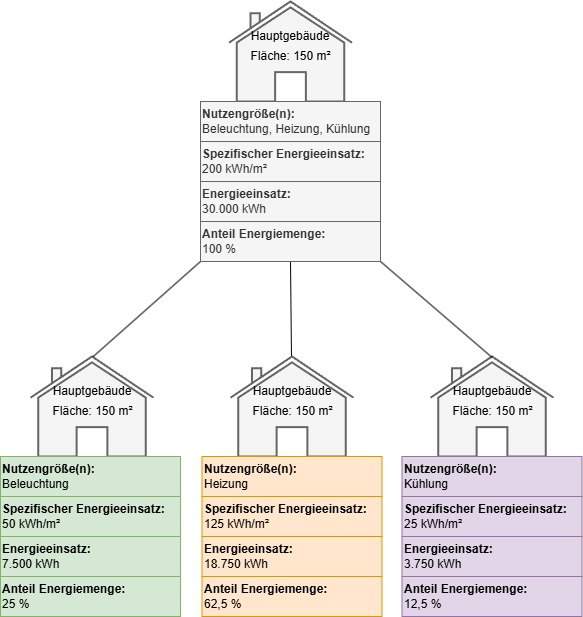
\includegraphics[width=1\textwidth]{../../Ressourcen/Abbildungen/Nutzengröße_Bewertungseinheit_Zerlegt_Beispiel.jpg}
    \caption{Beispiel: Disaggregation nach Nutzengrößen. (Eigene Darstellung)}
    \label{fig:Disagggregation_Bilanzraum_Nutzengrößen_Beispiel}
\end{figure}

Abbildung \eqref{fig:Disagggregation_Bilanzraum_Nutzengrößen_Beispiel} zeigt Beispielhaft wie das erarbeitete Konzept von Bilanzräumen zum erkennen von 
wesentlichen Energieeinsätzen beitragen kann. Wenn die aufwandsseitigen Ressourcen in einem festglegten Zeitintervall bekannt sind und die Nutzengröße durch eine 
Bewertungseinheit, wie in diesem Fall der Grundfläche in m², kann daraus mithilfe der Gleichung \eqref{SepzifischerEnergieinsatzMiller} der spezifische 
Energieeinsatz ermittelt werden. 
Unter Verwendung der Gleichung \eqref{EnergieeinsatzMiller} kann der Energieeinsatz im festglegten Zeitintervall berechnet werden und über den Anteil am 
gesamten Energieeinsatz von anderen Unterbilanzräumen unterschieden werden.
In diesem Beispiel macht die Heizungsanlage des Hauptgebäudes mit einem Energieeinsatz von 18.750 kWh 62,5 \% des Gesamtenergieverbrauchs aus und hat somit einen 
wesentlich Größeren Anteil am Gesamtenergieverbrauch als die Kühlungsanlage des Hauptgebäudes, welche mit einem Energieeinsatz von 3.750 kWh nur 12,5 \% des 
Gesamtenergieverbrauchs ausmacht.
Ob beim Energieeinsatz der Heizungsanlage ein erhebliches Potential für eine Verbesserung der energiebezogenen Leistung hat besteht hängt von den 
Anlagentechnischen Gegebenheiten der Heizung und den Gebäudetechnischen Gegebenheitung, wie Wärmedämmung ab.

Außerdem kann eine Analyse der Standorte beziehungsweise Gebäudezonen durch Disagggregation nach Untersuchungsgegenstand wie sie in 
\eqref{fig:Disagggregation_Bilanzraum_Untersuchungsgegenstand} visualisiert ist zur Identifikation wesentlicher Energieeinsätze durch die Analyse und Unterscheidung 
von Energieeinsätzen innerhalb von Gebäude(-zonen) beitragen.
\begin{figure}[H]
    \centering
    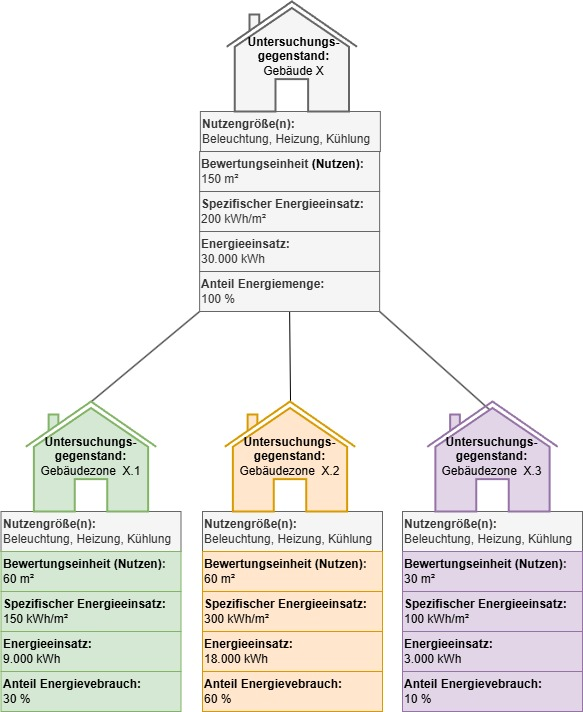
\includegraphics[width=1\textwidth]{../../Ressourcen/Abbildungen/Untersuchungsgegenstand_Zerlegt_Beispiel.jpg}
    \caption{Beispiel: Disaggregation nach Untersuchungsgegenstand. (Eigene Darstellung)}
    \label{fig:Disagggregation_Bilanzraum_Untersuchungsgegenstand_Beispiel}
\end{figure}
Abbildung \eqref{fig:Disagggregation_Bilanzraum_Untersuchungsgegenstand_Beispiel} visualisiert beispielhaft, wie eine Disagggregation des Untersuchungsgegenstands 
zur Analyse und Unterscheidung von Energieeinsätzen aus einer Perspektive des Standorts, also des Gebäudes und dessen Gebäudezonen, beitragen kann.
In diesem Beispiel macht die Etage 2 mit einem Energieeinsatz von 18.000 kWh 60\% des Gesamtenergieverbrauchs des Gebäudes aus während Etage 3 mit 
einem Energieeinsatz von 3.000 kWh nur 10\% des Gesamtenergieverbrauchs ausmacht.
Auch bei dieser Art der Disagggregation hängt das Potential für eine Verbesserung der energiebezogenen Leistung von den Gegebenheiten vor Ort ab.
Man sieht allerdings am Spezifischen Energieeinsatz, welcher die Größe der Grundfläche der Gebäudezonen mit einbezieht, dass in Etage 2 mit 300 kWh/m² 
im Verhältnis zu den anderen beiden Gebäudezonen ein hoher Spezifischer Energieeinsatz besteht. 
Das bedeutet dass Pro m² viel Energie verbraucht wird und kann ein Potential zur Verbesserung der energiebezogenen Leistung implizieren.

\subsubsection{Datengetriebene Ermittlung von Energieeinsätzen}

Bei der Implementation eines Energiemanagementsystems sind sowohl technologische als auch menschliche Aspekte zu beachten (\cite[S. 3]{Szajdzicki.2017}).
Die DIN EN ISO 50001:2018-12 fordert von Organisationen welche die Norm umsetzen möchten dass ein Plan zu Überwachung und Messung der Hauptmerkmale auf 
menschlicher Seite erstellt und dokumentiert wird und auf technischer Seite umgesetzt wird (\cite[S. 30ff.]{DIN50001.2018}).
Um die genauen Vorgaben der DIN EN ISO 50001:2018-12 zur ermittlung von Energieeinsätzen zu formulieren, wurde die E DIN ISO 50006:2024-07 veröffentlicht,
welche sich mit der Messung der energiebezogenen Leistung im Rahmen der DIN EN ISO 50001:2018-12 befasst (\cite[S. 1]{DIN50006.2024}).
Organisationen sollen nach E DIN ISO 50006:2024-07 (Kapitel 5.1) Arten des Energieeinsatzes identifizieren und zum einen deren aktuellen, sowie früheren 
Energieverbrauch, zum anderen die aktuelle und frühere Energieeffizienz auf Basis von Messungen und anderen Daten bewerten. 
SEUs werden dann anhand der Analyse dieser Informationen, unter berücksichtigung von Faktoren die die energiebezogene Leistung beeinflussen, 
identifiziert (\cite[Kapitel 5.1]{DIN50006.2024}). 

Die Datengetriebenen Ermittlung von Energieeinsätzen in Bilanzräumen fordert somit die Energiedatensammlung der aufwandsseitigen Ressourcen, zu der auch die DIN EN ISO 50001:2018-12 Vorgaben macht.
Die DIN EN ISO 50001:2018-12 (2018, Kapitel 6.6, A.6.6) stellt Anforderungen und Qualitätskriterien an die Datensammlung in Organisationen.
Die Norm verpflichtet Organisationen dazu, Hauptmerkmale ihrer Tätigkeiten, die sich auf die energiebezogene Leistung auswirken, zu identifizieren und diese in geplanten
Zeitabständen zu messen, zu überwachen und zu analysieren (\cite[S. 23]{DIN50001.2018}).
Teil der zu erfassenden Hauptmerkmale ist der Energieverbrauch bezüglich wesentlicher Energieeinsätze (\cite[S. 23]{DIN50001.2018}). 
Die Komplexität der Umsetzung ist dabei nicht vorgeschrieben und kann von einfachen Zählwerten bis hin zu umfangreichen Werten aus Überwachungs- und Messsystemen mit
Softwareanwendung reichen (\cite[S. 36]{DIN50001.2018}).
Aus Gleichung \eqref{SepzifischerEnergieinsatzMiller} folgt dass ohne die Erfassung der aufwandsseitigen Ressourcen einer Nutzengröße keine Berechnung des 
Energieeinsatzes möglich ist. 
Folglich bestimmt die Komplexität der Energiedatensammlung auch die potentielle Komplexität der Abbildung und Energiebilanzierung 
des Organisationskontext über Bilanzräume. 

Zusätztlich zu den Vorgaben über den Umfang der Energiedatensammlung gibt die DIN EN ISO 50001:2018-12 auch Qualitätskriterien der Energiedatensammlung vor.
So muss eine geeignete Abtastzeit der Datensammlung gewählt werden (\cite[S. 20]{DIN50006.2024}),und im Rahmen von Analysen müssen Einschränkungen der Daten 
wie Genauigkeit, Präzision und Konsistenz der Energiedatenerfassung Rechnung getragen werden (\cite[S. 37]{DIN50001.2018}).  
Da sich die DIN EN ISO 50001:2018-12 auf die Veränderung der energiebezogenen Leistung bezieht ist die Wiederholbarkeit ein wichtigeres Qualitätskriterium der 
Energiedatensammlung als die Präzision der Messung (\cite[S. 3]{Szajdzicki.2017}).

\subsubsection{Datengetriebene Ermittlung von relevanten Variablen}

Zur ermittlung wesentlicher Energieeinsätze ist nicht nur die Messung deren Energieverbrauchs notwendig, sondern auch die Messung und Überwachung der relevanten Variablen 
bezüglich SEUs (\cite[S. 23]{DIN50001.2018}). 
Relevante Variablen werden von der DIN EN ISO 50001:2018-12 (Kapitel 3.4.9) als quantifizierbarer Faktor, der die energiebezogene Leistung wesentlich beeinflusst sich 
routinemäßig ändert definiert. 
Beispiele für relevante Variablen für SEUs sind Wetterbedingungen, Betriebsbedingungen wie Innenraumtemperatur oder Lichtstärke und Arbeitsstunden (\cite[Kapitel 3.4.9]{DIN50001.2018}).
Die relevanten Variablen dürfen gemäß E DIN ISO 50006:2024-07 entweder direkt gemessen oder aus Messungen abgeleitet werden (\cite[S. 18]{DIN50006.2024}).